\documentclass[12pt,a4paper]{report}

% ============================================================================
% PACKAGES
% ============================================================================
\usepackage[utf8]{inputenc}
\usepackage[T1]{fontenc}
\usepackage{lmodern}
\usepackage[margin=1in]{geometry}
\usepackage{graphicx}
\usepackage{xcolor}
\usepackage{hyperref}
\usepackage{tikz}
\usepackage{longtable}
\usepackage{booktabs}
\usepackage{fancyhdr}
\usepackage{titlesec}
\usepackage{listings}
\usepackage{enumitem}

% TikZ Libraries
\usetikzlibrary{shapes.geometric, arrows.meta, positioning, fit, backgrounds}

% ============================================================================
% COLORS
% ============================================================================
\definecolor{primaryblue}{RGB}{26, 54, 93}
\definecolor{secondaryblue}{RGB}{59, 130, 246}
\definecolor{accentgreen}{RGB}{34, 197, 94}
\definecolor{warningorange}{RGB}{249, 115, 22}
\definecolor{dangerred}{RGB}{239, 68, 68}
\definecolor{lightgray}{RGB}{243, 244, 246}
\definecolor{darkgray}{RGB}{75, 85, 99}
\definecolor{purplegrade}{RGB}{139, 92, 246}

% ============================================================================
% HYPERREF SETUP
% ============================================================================
\hypersetup{
    colorlinks=true,
    linkcolor=primaryblue,
    urlcolor=secondaryblue,
    pdftitle={EduX - Examination System Guide},
    pdfauthor={EduX Development Team},
}

% ============================================================================
% HEADER/FOOTER
% ============================================================================
\pagestyle{fancy}
\fancyhf{}
\fancyhead[L]{\textcolor{darkgray}{\small EduX School Management System}}
\fancyhead[R]{\textcolor{darkgray}{\small Examination Guide}}
\fancyfoot[C]{\textcolor{darkgray}{\thepage}}
\renewcommand{\headrulewidth}{0.4pt}

% ============================================================================
% TITLE FORMATTING
% ============================================================================
\titleformat{\chapter}[display]
  {\normalfont\huge\bfseries\color{primaryblue}}
  {\chaptertitlename\ \thechapter}{20pt}{\Huge}

\titleformat{\section}
  {\normalfont\Large\bfseries\color{primaryblue}}
  {\thesection}{1em}{}

\titleformat{\subsection}
  {\normalfont\large\bfseries\color{secondaryblue}}
  {\thesubsection}{1em}{}

% ============================================================================
% DOCUMENT
% ============================================================================
\begin{document}

% ----------------------------------------------------------------------------
% TITLE PAGE
% ----------------------------------------------------------------------------
\begin{titlepage}
    \centering
    \vspace*{2cm}
    
    {\Huge\bfseries\textcolor{primaryblue}{EduX}\par}
    \vspace{0.5cm}
    {\Large\textcolor{secondaryblue}{School Management System}\par}
    
    \vspace{2cm}
    
    
\begin{tikzpicture}
        \node[draw=primaryblue, line width=2pt, rounded corners=10pt, 
              minimum width=8cm, minimum height=3cm, fill=lightgray] 
              {\Huge\bfseries\textcolor{primaryblue}{Examination System}};
    \end{tikzpicture}
    
    \vfill
    
    {\large\textcolor{darkgray}{Version 1.0}\par}
    {\large\textcolor{darkgray}{\today}\par}
\end{titlepage}

\tableofcontents
\newpage

% ============================================================================
% CHAPTER 1: OVERVIEW
% ============================================================================
\chapter{Examination System Overview}

\section{Introduction}

The Examination module manages the complete exam lifecycle from creation to report card generation.

\section{Exam Workflow}

\begin{center}
\begin{tikzpicture}[
    node distance=0.8cm,
    step/.style={draw=primaryblue, rounded corners, minimum width=4cm, 
                 minimum height=1cm, fill=lightgray, align=center, font=\small},
    arrow/.style={-{Stealth}, thick, secondaryblue}
]
    \node[step] (s1) {Create Exam};
    \node[step, below=of s1] (s2) {Add Subjects};
    \node[step, below=of s2] (s3) {Schedule Dates};
    \node[step, below=of s3] (s4) {Enter Marks};
    \node[step, below=of s4] (s5) {Calculate Results};
    \node[step, below=of s5] (s6) {Generate Report Cards};
    
    \draw[arrow] (s1) -- (s2);
    \draw[arrow] (s2) -- (s3);
    \draw[arrow] (s3) -- (s4);
    \draw[arrow] (s4) -- (s5);
    \draw[arrow] (s5) -- (s6);
\end{tikzpicture}
\end{center}

\section{Exam Types}

\begin{center}

\begin{tikzpicture}[
    type/.style={draw=purplegrade, rounded corners, minimum width=2.8cm, 
                 minimum height=0.9cm, fill=purplegrade!10, font=\small\bfseries, 
                 text=purplegrade}
]
    \node[type] (unit) at (0,0) {Unit Test};
    \node[type, right=0.3cm of unit] (monthly) {Monthly Test};
    \node[type, right=0.3cm of monthly] (term) {Term Exam};
    \node[type, right=0.3cm of term] (annual) {Annual Exam};
\end{tikzpicture}
\end{center}

% ============================================================================
% CHAPTER 2: CREATING EXAMS
% ============================================================================
\chapter{Creating Exams}

\section{Exam Creation}

Navigate to \texttt{Exams} $\rightarrow$ \texttt{Create Exam}

\begin{longtable}{@{}p{4cm}p{3cm}p{6cm}@{}}
\toprule
\textbf{Field} & \textbf{Required} & \textbf{Description} \\
\midrule
\endhead
Exam Name & Yes & e.g., ``First Term Exam 2025'' \\
Exam Type & Yes & Unit Test / Term Exam / Annual \\
Class & Yes & Target class \\
Academic Year & Yes & Current academic year \\
Start Date & Yes & Exam period start \\
End Date & No & Exam period end \\
Description & No & Additional details \\
\bottomrule
\end{longtable}

\section{Adding Exam Subjects}

For each subject in the exam:

\begin{longtable}{@{}p{4cm}p{3cm}p{6cm}@{}}
\toprule
\textbf{Field} & \textbf{Required} & \textbf{Description} \\
\midrule
\endhead
Subject & Yes & Select from class subjects \\
Maximum Marks & Yes & Total marks (e.g., 100) \\
Passing Marks & Yes & Minimum to pass (e.g., 33) \\
Exam Date & No & Date of this subject exam \\
Exam Time & No & Start time \\
Duration & No & Duration in minutes \\
\bottomrule
\end{longtable}

\section{Exam Status}

\begin{center}

\begin{tikzpicture}[
    state/.style={draw=#1, rounded corners, minimum width=2.5cm, 
                  minimum height=1cm, fill=#1!15, font=\small\bfseries, text=#1}
]
    \node[state=warningorange] (draft) at (0,0) {Draft};
    \node[state=secondaryblue, right=1cm of draft] (active) {Active};
    \node[state=accentgreen, right=1cm of active] (completed) {Completed};
    
    \draw[-{Stealth}, thick] (draft) -- node[above, font=\scriptsize] {publish} (active);
    \draw[-{Stealth}, thick] (active) -- node[above, font=\scriptsize] {finalize} (completed);
\end{tikzpicture}
\end{center}

% ============================================================================
% CHAPTER 3: MARKS ENTRY
% ============================================================================
\chapter{Marks Entry}

\section{Entering Marks}

Navigate to \texttt{Exams} $\rightarrow$ Select Exam $\rightarrow$ \texttt{Enter Marks}

\begin{enumerate}[leftmargin=*]
    \item Select exam
    \item Select subject
    \item View student list
    \item Enter marks for each student
    \item Mark absent students (checkbox)
    \item Save marks
\end{enumerate}

\section{Marks Entry Grid}

\begin{center}
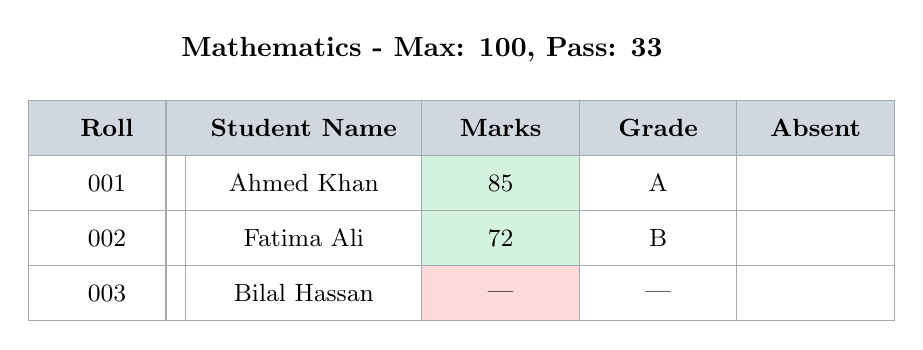
\begin{tikzpicture}[
    cell/.style={minimum width=2cm, minimum height=0.7cm, draw=darkgray!50, 
                 font=\small},
    header/.style={cell, fill=primaryblue!20, font=\small\bfseries}
]
    % Subject header
    \node[font=\bfseries] at (4,1) {Mathematics - Max: 100, Pass: 33};
    
    % Headers
    \node[header] at (0,0) {Roll};
    \node[header, minimum width=3.5cm] at (2.5,0) {Student Name};
    \node[header] at (5,0) {Marks};
    \node[header] at (7,0) {Grade};
    \node[header] at (9,0) {Absent};
    
    % Row 1
    \node[cell] at (0,-0.7) {001};
    \node[cell, minimum width=3.5cm] at (2.5,-0.7) {Ahmed Khan};
    \node[cell, fill=accentgreen!20] at (5,-0.7) {85};
    \node[cell] at (7,-0.7) {A};
    \node[cell] at (9,-0.7) {$\square$};
    
    % Row 2
    \node[cell] at (0,-1.4) {002};
    \node[cell, minimum width=3.5cm] at (2.5,-1.4) {Fatima Ali};
    \node[cell, fill=accentgreen!20] at (5,-1.4) {72};
    \node[cell] at (7,-1.4) {B};
    \node[cell] at (9,-1.4) {$\square$};
    
    % Row 3
    \node[cell] at (0,-2.1) {003};
    \node[cell, minimum width=3.5cm] at (2.5,-2.1) {Bilal Hassan};
    \node[cell, fill=dangerred!20] at (5,-2.1) {---};
    \node[cell] at (7,-2.1) {---};
    \node[cell] at (9,-2.1) {$\boxtimes$};
\end{tikzpicture}
\end{center}

\section{Validation Rules}

\begin{itemize}[leftmargin=*]
    \item Marks cannot exceed maximum marks
    \item Either marks or absent must be specified
    \item Automatic grade calculation based on grade settings
    \item Warning for marks below passing
\end{itemize}

% ============================================================================
% CHAPTER 4: GRADING SYSTEM
% ============================================================================
\chapter{Grading System}

\section{Grade Configuration}

Navigate to \texttt{Exams} $\rightarrow$ \texttt{Grade Settings}

\begin{center}
\begin{tikzpicture}
    % Title
    \node[font=\bfseries] at (4,4) {Default Grading Scale};
    
    % Headers
    \fill[primaryblue!20] (0,3) rectangle (8,3.5);
    \node[font=\small\bfseries] at (1,3.25) {Grade};
    \node[font=\small\bfseries] at (3,3.25) {Min \%};
    \node[font=\small\bfseries] at (5,3.25) {Max \%};
    \node[font=\small\bfseries] at (7,3.25) {GPA};
    
    % Grades
    \foreach \y/\grade/\min/\max/\gpa/\color in {
        2.5/A+/90/100/4.0/accentgreen,
        2/A/80/89/3.7/accentgreen,
        1.5/B+/70/79/3.3/secondaryblue,
        1/B/60/69/3.0/secondaryblue,
        0.5/C/50/59/2.5/warningorange,
        0/D/33/49/2.0/warningorange
    } {
        \fill[\color!10] (0,\y) rectangle (8,\y+0.5);
        \node[font=\small\bfseries, text=\color] at (1,\y+0.25) {\grade};
        \node[font=\small] at (3,\y+0.25) {\min\%};
        \node[font=\small] at (5,\y+0.25) {\max\%};
        \node[font=\small] at (7,\y+0.25) {\gpa};
    }
    
    \fill[dangerred!10] (0,-0.5) rectangle (8,0);
    \node[font=\small\bfseries, text=dangerred] at (1,-0.25) {F};
    \node[font=\small] at (3,-0.25) {0\%};
    \node[font=\small] at (5,-0.25) {32\%};
    \node[font=\small] at (7,-0.25) {0.0};
    
    \draw[primaryblue] (0,-0.5) rectangle (8,3.5);
\end{tikzpicture}
\end{center}

\section{Adding Custom Grades}

\begin{enumerate}[leftmargin=*]
    \item Click \texttt{Add Grade}
    \item Enter grade name (e.g., ``A+'')
    \item Set minimum and maximum percentage
    \item Enter GPA points
    \item Add remarks (shown on report card)
    \item Set display order
    \item Mark as passing/failing grade
\end{enumerate}

% ============================================================================
% CHAPTER 5: RESULTS
% ============================================================================
\chapter{Results \& Analysis}

\section{Result Calculation}

After all marks are entered:
\begin{enumerate}[leftmargin=*]
    \item Go to exam details
    \item Click \texttt{Calculate Results}
    \item System computes:
    \begin{itemize}
        \item Total marks obtained
        \item Percentage
        \item Overall grade
        \item GPA
        \item Class rank
        \item Pass/Fail status
    \end{itemize}
    \item Review and confirm
\end{enumerate}

\section{Result Summary}

\begin{center}
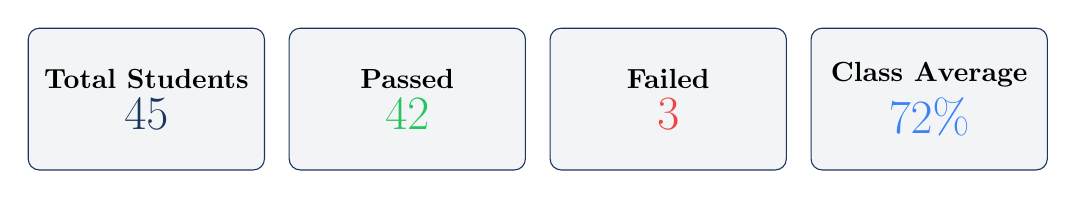
\begin{tikzpicture}[
    stat/.style={draw=primaryblue, rounded corners, minimum width=3cm, 
                 minimum height=1.8cm, fill=lightgray, align=center}
]
    \node[stat] (total) at (0,0) {
        \textbf{Total Students}\\[0.1cm]
        \textcolor{primaryblue}{\LARGE 45}
    };
    \node[stat, right=0.3cm of total] (passed) {
        \textbf{Passed}\\[0.1cm]
        \textcolor{accentgreen}{\LARGE 42}
    };
    \node[stat, right=0.3cm of passed] (failed) {
        \textbf{Failed}\\[0.1cm]
        \textcolor{dangerred}{\LARGE 3}
    };
    \node[stat, right=0.3cm of failed] (avg) {
        \textbf{Class Average}\\[0.1cm]
        \textcolor{secondaryblue}{\LARGE 72\%}
    };
\end{tikzpicture}
\end{center}

\section{Subject-wise Analysis}

View performance across subjects:
\begin{itemize}[leftmargin=*]
    \item Highest/Lowest scores
    \item Class average per subject
    \item Pass percentage per subject
    \item Grade distribution charts
\end{itemize}

% ============================================================================
% CHAPTER 6: REPORT CARDS
% ============================================================================
\chapter{Report Cards}

\section{Generating Report Cards}

Navigate to \texttt{Exams} $\rightarrow$ Select Exam $\rightarrow$ \texttt{Report Cards}

\begin{enumerate}[leftmargin=*]
    \item Select exam(s) to include
    \item Choose students (all or specific)
    \item Add teacher remarks (optional)
    \item Add principal remarks (optional)
    \item Preview report cards
    \item Print or export as PDF
\end{enumerate}

\section{Report Card Layout}

\begin{center}
\begin{tikzpicture}[
    box/.style={draw=primaryblue, minimum width=8cm, align=left, font=\small}
]
    \node[box, minimum height=8cm, fill=lightgray] at (0,0) {
        \centering\textbf{\large SCHOOL NAME}\\
        \textit{Report Card}\\[0.3cm]
        \rule{7.5cm}{0.4pt}\\[0.2cm]
        \textbf{Student:} Ahmed Khan \hfill \textbf{Class:} 5A\\
        \textbf{Roll No:} 001 \hfill \textbf{Exam:} Annual 2025\\[0.2cm]
        \rule{7.5cm}{0.4pt}\\[0.2cm]
        \begin{tabular}{lrrr}
        \textbf{Subject} & \textbf{Max} & \textbf{Obtained} & \textbf{Grade}\\
        English & 100 & 85 & A\\
        Mathematics & 100 & 78 & B+\\
        Science & 100 & 82 & A\\
        Urdu & 100 & 75 & B+\\
        Islamiat & 50 & 42 & A\\
        \end{tabular}\\[0.2cm]
        \rule{7.5cm}{0.4pt}\\[0.2cm]
        \textbf{Total:} 362/450 \hfill \textbf{Percentage:} 80.4\%\\
        \textbf{Grade:} A \hfill \textbf{Rank:} 5\\[0.2cm]
        \rule{7.5cm}{0.4pt}\\[0.2cm]
        \textbf{Remarks:} Excellent performance!\\[0.3cm]
        \rule{3cm}{0.4pt} \hfill \rule{3cm}{0.4pt}\\
        Class Teacher \hfill Principal
    };
\end{tikzpicture}
\end{center}

\section{Bulk Printing}

\begin{enumerate}[leftmargin=*]
    \item Select all students or filter by section
    \item Click \texttt{Print All}
    \item Configure print settings
    \item Print batch of report cards
\end{enumerate}

% ============================================================================
% CHAPTER 7: EXAM REPORTS
% ============================================================================
\chapter{Exam Reports}

\section{Available Reports}

\begin{longtable}{@{}p{4cm}p{9cm}@{}}
\toprule
\textbf{Report} & \textbf{Description} \\
\midrule
\endhead
Result Sheet & Complete marks for all students \\
Grade Distribution & Students per grade category \\
Subject Analysis & Performance by subject \\
Toppers List & Rank-wise student list \\
Failed List & Students who failed \\
Comparative Report & Compare across exams \\
\bottomrule
\end{longtable}

\section{Export Options}

\begin{itemize}[leftmargin=*]
    \item \textbf{PDF} -- Formatted report with school header
    \item \textbf{Excel} -- Raw data for further analysis
    \item \textbf{Print} -- Direct printing
\end{itemize}

\end{document}
